\appendix
\chapter{Introduction to Machine Learning}\label{appx:introMachineLearning}

\section{Heaviside Function}\label{appx:sec:heaviside}

The Heaviside step function is defined as
\begin{equation}\label{eq:heavisideDefintion}
h(z) =
\begin{cases}
&0 \ \mbox{if} \ z<0 \\
&\frac{1}{2} \ \mbox{if} \ z=0 \\
&1 \ \mbox{if} \ z>0.
\end{cases}
\end{equation}

and the relation between the logistic function and the heaviside function is
\begin{equation}
 \ H(z) = \lim_{k \to \infty} \left(\frac{1}{2} + \frac{1}{2}\tanh(kz) \right) = \lim_{k \to \infty} \left(\frac{1}{1+e^{-kz}} \right)
\end{equation}

Note in this sense that for a binary classification problem, the heaviside function \cref{eq:heavisideDefintion} is more appealing to the task, although its singularity at $z=0$ is problematic for optimization routines.

\section{Details of the log loss functions}\label{appx:sec:loglossDetails}

In \cref{figure-logLossValues} we display the values of the log loss function for different input probabilities:

\begin{figure}[h!]
\begin{center}
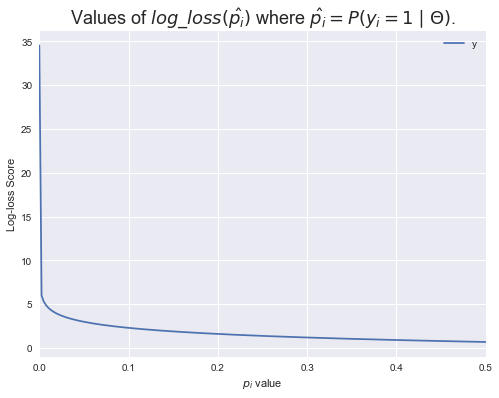
\includegraphics[width=0.7\columnwidth]{figures/logloss/figure-logLossValues.png}
\caption{ Error score series plot for the log loss function.
Different $p_i$ input values are displayed with their output log loss score.}
\label{figure-logLossValues}
\end{center}
\end{figure}

From what is shown, the function is heavier for small probability values near zero than it is positive for large values near one.
This means that it penalizes strongly on wrong predictions; samples where the algorithm has a strong confidence in the prediction yet has misclassified.
This properties can be taken into advantage during the optimization procedure, which will always converge to a global optima.

Also, explicit forms can be given for the gradient and the Hessian of the loss function with regard to the whole dataset $X$ as a sum involving individual samples $x$.

The negative gradient can be analytically expressed in the following way: %can thus be analytically expressed
\begin{equation}
- \nabla l(\theta) = \sum_{i=1}^N (y_i - P(y_i \mid x_i,\theta))\cdot x_i = \textbf{X}^{\intercal}(\textbf{y}-\textbf{p})
\label{eq:logitHessian1}
\end{equation}
whilst the Hessian takes the following form:
\begin{equation}
\frac{\partial^2 l(\theta)}{\partial \theta \partial \theta^\intercal} = \sum_{i=1}^N x_i \cdot x_i^\intercal P(y_i \mid x_i,\theta)(1 -P(y_i \mid x_i,\theta))
\label{eq:logitHessian2}
\end{equation}

With this formulation, we can take any optimization procedure that benefits from the closed-form representations of the first and second derivatives of the loss function.



\chapter{Model Selection}

\section{Extension of bias and variance to other loss functions}\label{appx:sec:biasVarianceExtensionLoss}

adsfas

